\documentclass{style/tongjithesis}
\usepackage{style/tongjithesis}
\begin{document}

\pagestyle{firststyle}
%%%%%%%%%%%%%%%%%%%%%%%%%%%%%%%%%%%%%%%%
\MakeAbstract{
    同济大学(英语:Tongji University),简称同济,是位于中国上海市的一所综合性大学,是中华人民共和国教育部直属的全国重点大学,行政级别为副部级,是“双一流A类”和原“985工程”、原“211工程”重点建设大学,同时是卓越大学联盟、全球环境与可持续发展合作联盟(GUPES)、国际设计艺术院校联盟(Cumulus)、21世纪学术联盟(AC21)、同济-伯克利工程联盟(Tongji-Berkeley Alliance)、中俄工科大学联盟(ASRTU)成员。

    同济大学的前身是1907年创办的德文医学堂,后改名为同济德文医学堂;1912年与创办不久的同济德文工学堂合并,更名为同济德文医工学堂;1923年正式定名为同济大学;1927年成立国立同济大学,是中国最早的七所国立大学之一;1949年更名为同济大学。

    同济大学目前共设有38个学院(系)和二级办学机构,7家附属医院,5所附属中学;有全日制本科生1.7万余人,硕士研究生1.3万余人,博士研究生近5000人。有外国留学生数千人;学校占地面积约3850亩;纸本图书400余万册。

    根据2021年的QS世界大学排名和泰晤士高等教育世界大学排名,同济大学分别位列中国第九和第十六。
}{同济大学,上海,综合性大学,重点大学}

\MakeAbstractEng{
    Tongji University (Chinese: 同济大学) is a national public research university located in Shanghai. Established in 1907 by the German government together with German physicians in Shanghai, Tongji is one of the longest-standing, most selective, and most prestigious universities in China under the Project 985 and Double First Class University Plan. It is a Chinese state Class A Double First Class University.

    Tongji University is renowned for its architecture, engineering and business programs which consistently rank among the best in the world. Tongji's architecture program was rated the top overall architecture program in China according to China's University and College Admission System (CACUS) and ranks as the \nth{13} best architecture program in the world according to the QS World University Rankings. The College of Civil Engineering is considered the best in the world according to several widely cited international rankings, including Shanghai Ranking, U.S. News Rankings, URAP ranking and NTU Ranking. The U.S. News \& World Report Best Global University Ranking ranks Tongji University at \nth{15} worldwide in engineering. The School of Design and Innovation was ranked \nth{12} among art and design schools worldwide in 2022, and the top in Asia, according to the QS. The School of Economics and Management (Tongji SEM) is one of 74 business schools in the world being triple accredited by the European Quality Improvement System (EQUIS), the Association to Advance Collegiate Schools of Business (AACSB) and the Association of MBAs (AMBA). Tongji University is a member of the Yangtze Delta Universities Alliance and Asian-European Laotse Universities Network. According to the 2022 QS World University Rankings, Tongji University ranked \nth{8} nationally. Tongji University consistently features in the top \nth{300} global universities.
}{Tongji University, Shanghai, comprehensive university, key university}
%%%%%%%%%%%%
%%%%%%%%%%%%%%%%%%%%%%%%%%%%%%%%%%%%%%%%

\newpage
\tableofcontents   %放置目录
\newpage

\pagestyle{mainstyle}
\section{引言}\label{introduction}

\subsection{问题背景与陈述}

探究电信学院大学生应该如何内卷是一个很重要的问题。

这里展示一下如何在本项目中插入图片:

\begin{figure}[hb!]
    \centering
    \subfigure[目标检测]{
    \begin{minipage}[t]{0.22\linewidth}
    \centering
    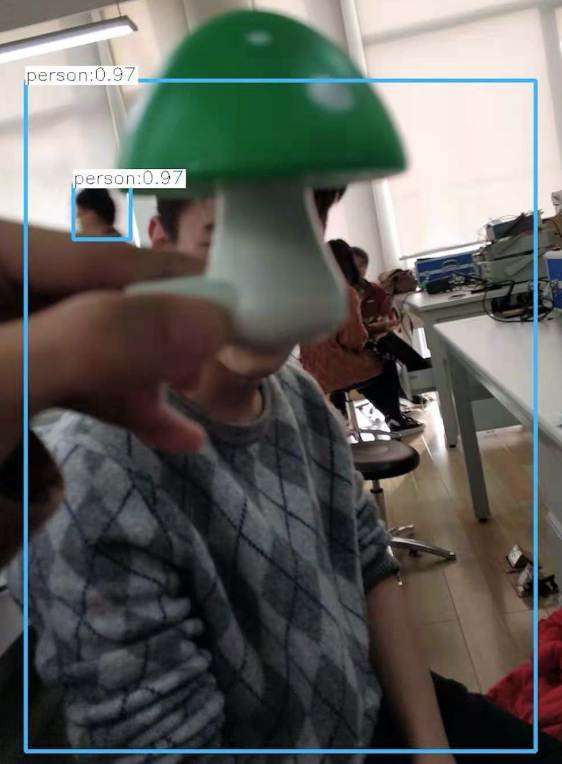
\includegraphics[width=\linewidth]{figures/det.png}
    \end{minipage}\label{fig:det}
    }
    %
    \centering
    \subfigure[语义分割]{
    \begin{minipage}[t]{0.28\linewidth}
    \centering
    
\includegraphics[width=\linewidth]{figures/seg.png}
    \end{minipage}\label{fig:seg}
    }
    %
    \centering
    \subfigure[姿态识别]{
    \begin{minipage}[t]{0.4\linewidth}
    \centering
    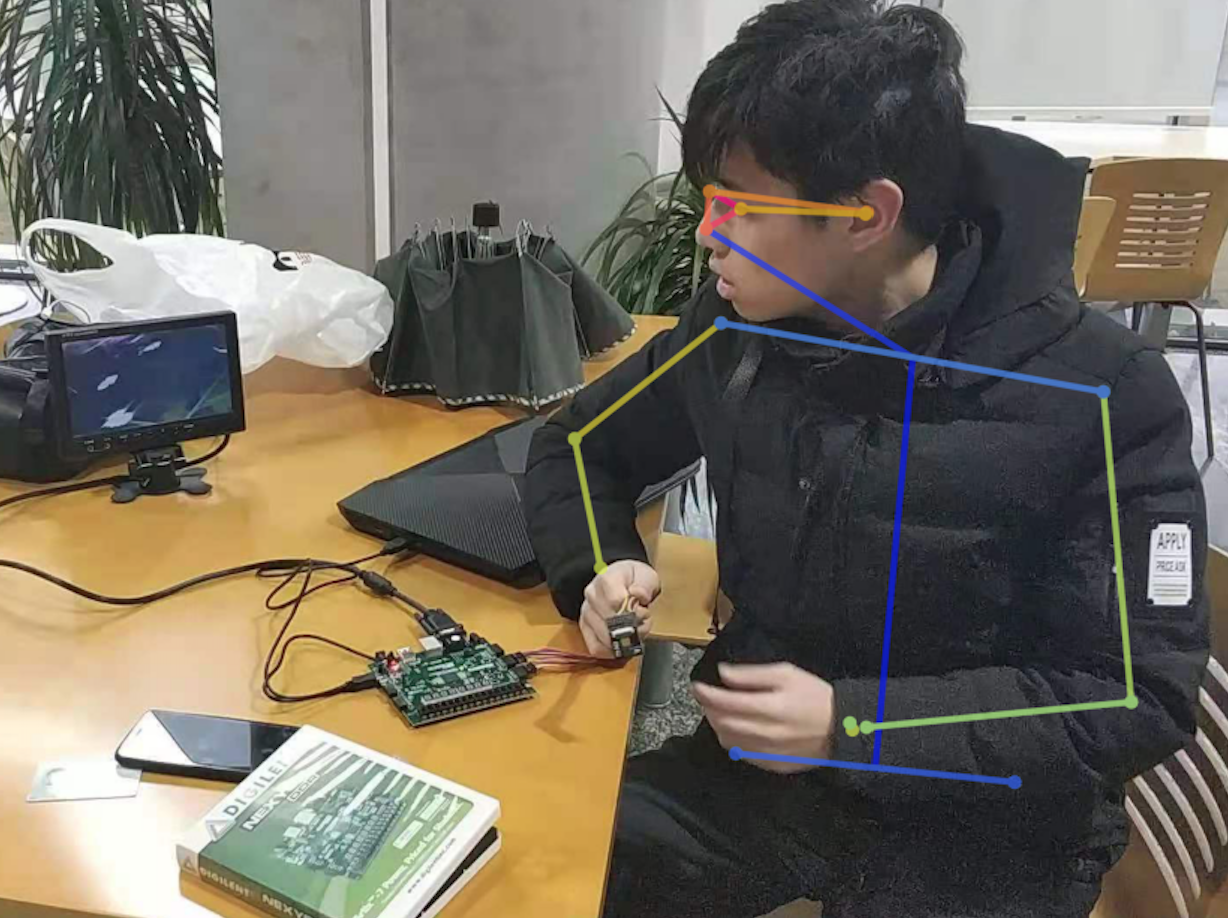
\includegraphics[width=\linewidth]{figures/pose.png}
    \end{minipage}\label{fig:pose}
    }
    %
    \caption{常见视频分析应用图解(图片提供者为中中同学)}\label{fig:cvexample}
    \centering
\end{figure}


\subsection{本文的工作}

本文的工作就是卷字数。

\subsection{文章结构}

采用递进式方法进行卷字数。

\newpage
\section{预备知识}\label{preliminaries}

\subsection{SOTA: 螺旋鲲鲲卷}

本节将介绍鲲鲲\cite{kun}是如何卷的。

\subsection{SOTA: 霹雳中中卷}

本节将介绍中中\cite{zhong}是如何卷的。

\newpage
\section{算法设计}\label{algorithm}

\subsection{伟伟卷卷法}

\subsubsection{电竞法}

每天12小时的英雄联盟游戏时间。

\subsubsection{追剧法}

每天再抽12小时看Netflix。

\newpage
\section{实验比较}\label{numerical experiments}

\subsection{内卷竞赛}

本节分别使用鲲鲲内卷法,中中内卷法,伟伟内卷法进行时间比较。在3天内,让实验组和对照组分别在3天内写论文。鲲鲲卷卷法3天写出了一篇CVPR,中中卷卷法3天写出了一篇AAAI,对照组三天写出了一份10页报告,而伟伟卷卷法3天从黄铜上分到了白银。

\newpage
\section{总结与未来工作展望}\label{conclusion}

写下你的未来工作展望。

\newpage

\addcontentsline{toc}{section}{参考文献}
\bibliography{note}

\newpage
\section*{谢\ 辞}
\addcontentsline{toc}{section}{谢辞}

本节通常用于感谢在研究过程中给予帮助和支持的人们,例如指导老师、实验室同学、朋友和家人等。

在谢辞中,需要真诚地表达感谢之情,回顾一下在研究过程中所受到的帮助和支持,并提到他们的具体贡献和重要性。同时,也可以简要说明一下自己在研究过程中的收获和体会,表达对他们的感激之情和祝福。

最后,需要注意不要出现太多的感情用词,语言简洁明了,表达真诚和诚恳即可。

谢谢支持本项目的所有朋友们。并且希望选用该模板的朋友们都能顺利通过查重与答辩。


\end{document}
